% What is on the table.
%
% The point of the drawing is that there are two paths to the board and
% the project needs both at once: the serial line works when the kernel
% has stopped, and Ethernet is the only one that can move a trace file.
\documentclass[tikz, border=4pt]{standalone}
% Shared styles for the Project 9 figures.
%
% Every figure in this directory is standalone: it inputs this file and
% compiles on its own with
%
%     pdflatex arch.tex
%
% so a reader can render one drawing without building a book around it.
%
% The palette carries the distinction this project keeps confusing when it
% is drawn in one colour: what runs on the target, what runs on the host,
% and which of the two halves of the serial cable a given box is talking
% to. The fourth colour is for a fault that produces no symptom, which is
% three of the four faults here and the reason the project exists.
\usepackage{tikz}
\usepackage[siunitx]{circuitikz}
\usetikzlibrary{arrows.meta, backgrounds, calc, fit, positioning, shapes.geometric, shapes.misc}

\definecolor{usercol}{RGB}{222, 235, 247}   % target, user space
\definecolor{kerncol}{RGB}{198, 219, 239}   % target, kernel
\definecolor{hostcol}{RGB}{229, 245, 224}   % host, off the board
\definecolor{toolcol}{RGB}{254, 217, 118}   % a debugging tool
\definecolor{hwcol}{RGB}{229, 229, 229}     % hardware, files, RAM
\definecolor{quietcol}{RGB}{245, 245, 245}  % a fault with no symptom
\definecolor{linecol}{RGB}{70, 70, 70}
\definecolor{badcol}{RGB}{200, 60, 60}
\definecolor{okcol}{RGB}{60, 140, 70}

\tikzset{
  blk/.style   = {draw=linecol, rounded corners=2pt, align=center,
                  font=\sffamily\small, inner sep=4pt, minimum height=9mm},
  user/.style  = {blk, fill=usercol},
  kern/.style  = {blk, fill=kerncol},
  host/.style  = {blk, fill=hostcol},
  tool/.style  = {blk, fill=toolcol},
  hw/.style    = {blk, fill=hwcol},
  quiet/.style = {blk, fill=quietcol, draw=linecol!50, dashed},
  bad/.style   = {blk, fill=white, draw=badcol, thick, text=badcol},
  layer/.style = {draw=linecol!40, dashed, rounded corners=3pt, inner sep=6pt},
  layerlabel/.style = {font=\sffamily\scriptsize\bfseries, inner sep=2pt},
  lbl/.style   = {font=\sffamily\scriptsize, fill=white, inner sep=1pt},
  flow/.style  = {-{Stealth[length=2mm]}, draw=linecol, thick},
  bus/.style   = {{Stealth[length=2mm]}-{Stealth[length=2mm]}, draw=linecol,
                  thick},
  % The serial line is drawn thick and dark everywhere it appears, because
  % the single point of this project's host side is that it is one wire.
  wire/.style  = {{Stealth[length=2mm]}-{Stealth[length=2mm]}, draw=linecol,
                  very thick},
  % UML sequence
  actor/.style = {blk, fill=usercol, font=\sffamily\scriptsize,
                  minimum height=6mm},
  lifeline/.style = {draw=linecol!50, dashed},
  msg/.style   = {-{Stealth[length=1.6mm]}, draw=linecol},
  reply/.style = {-{Stealth[length=1.6mm]}, draw=linecol, dashed},
  umlnote/.style = {draw=linecol!60, fill=yellow!12, rounded corners=1pt,
                    font=\sffamily\scriptsize, align=left, inner sep=3pt},
  activation/.style = {draw=linecol, fill=usercol, minimum width=2mm},
  % decision tree
  qst/.style   = {draw=linecol, fill=white, diamond, aspect=2.6, align=center,
                  font=\sffamily\scriptsize, inner sep=1pt},
  ans/.style   = {font=\sffamily\scriptsize\itshape, inner sep=1pt},
  fix/.style   = {blk, fill=hostcol, font=\sffamily\scriptsize, align=left},
  trans/.style = {-{Stealth[length=1.6mm]}, draw=linecol},
  % fault matrix
  cell/.style  = {draw=linecol!40, minimum width=17mm, minimum height=7mm,
                  font=\sffamily\scriptsize, align=center},
  hit/.style   = {cell, fill=okcol!25},
  miss/.style  = {cell, fill=badcol!12, text=badcol},
  head/.style  = {cell, font=\sffamily\scriptsize\bfseries, fill=hwcol},
}


\begin{document}
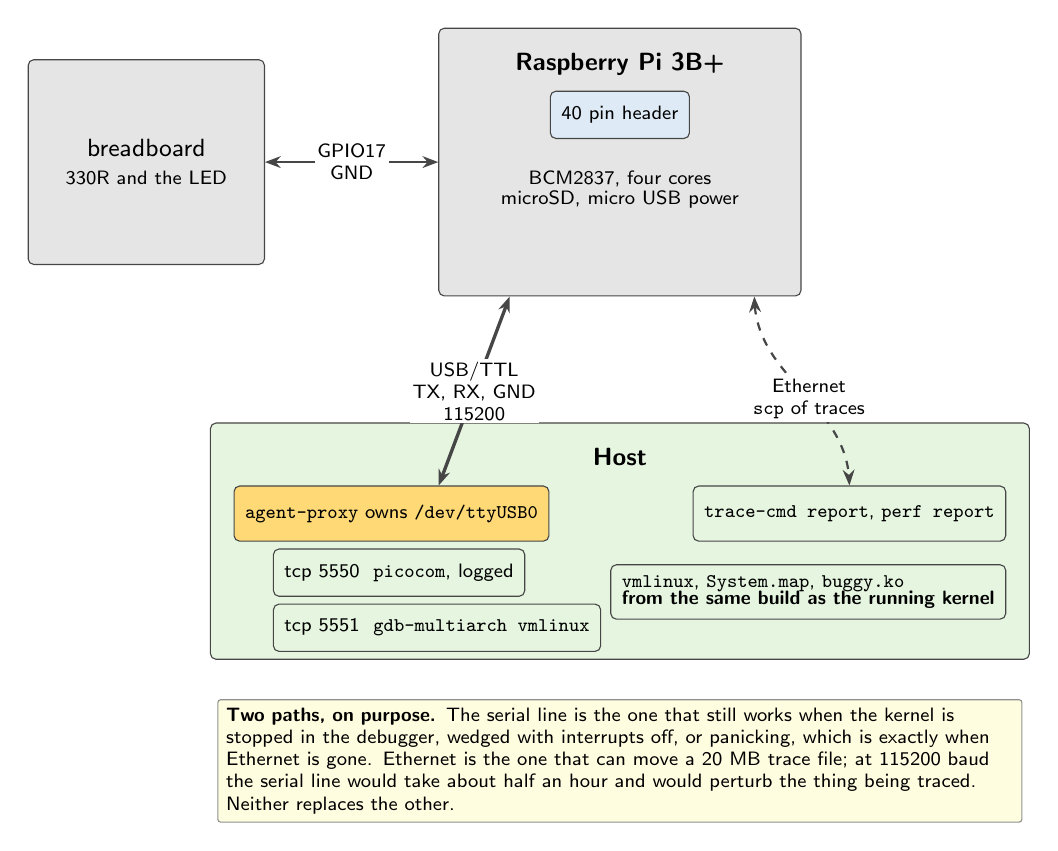
\begin{tikzpicture}[font=\sffamily\small, node distance=6mm]

  %% ---------------- breadboard ----------------
  \node[hw, minimum width=30mm, minimum height=26mm, align=center] (bb)
       {breadboard\\[-1pt]\scriptsize 330R and the LED};

  %% ---------------- the board ----------------
  \node[hw, right=22mm of bb, minimum width=46mm, minimum height=34mm,
        align=center] (pi) {};
  \node[font=\sffamily\small\bfseries, anchor=north]
       at ($(pi.north)+(0,-2mm)$) {Raspberry Pi 3B+};
  \node[user, anchor=north, minimum height=6mm, font=\sffamily\scriptsize]
       at ($(pi.north)+(0,-8mm)$) (hdr) {40 pin header};
  \node[font=\sffamily\scriptsize, anchor=north, align=center]
       at ($(pi.north)+(0,-17mm)$)
       {BCM2837, four cores\\[-1pt] microSD, micro USB power};

  \draw[bus] (bb.east) -- node[lbl, align=center]
       {GPIO17\\GND} (pi.west);

  %% ---------------- the two paths off the board ----------------
  \node[host, below=16mm of pi, minimum width=104mm, minimum height=30mm,
        align=center] (host) {};
  \node[font=\sffamily\small\bfseries, anchor=north]
       at ($(host.north)+(0,-2mm)$) {Host};

  \node[tool, anchor=north west, font=\sffamily\scriptsize, align=left,
        minimum height=7mm] at ($(host.north west)+(3mm,-8mm)$) (proxy)
       {\texttt{agent-proxy} owns \texttt{/dev/ttyUSB0}};
  \node[host, anchor=north west, font=\sffamily\scriptsize, align=left,
        minimum height=6mm] at ($(host.north west)+(8mm,-16mm)$) (t1)
       {tcp 5550 \ \texttt{picocom}, logged};
  \node[host, anchor=north west, font=\sffamily\scriptsize, align=left,
        minimum height=6mm] at ($(host.north west)+(8mm,-23mm)$) (t2)
       {tcp 5551 \ \texttt{gdb-multiarch vmlinux}};

  \node[host, anchor=north east, font=\sffamily\scriptsize, align=left,
        minimum height=7mm] at ($(host.north east)+(-3mm,-8mm)$) (rep)
       {\texttt{trace-cmd report}, \texttt{perf report}};
  \node[host, anchor=north east, font=\sffamily\scriptsize, align=left,
        minimum height=6mm] at ($(host.north east)+(-3mm,-18mm)$) (sym)
       {\texttt{vmlinux}, \texttt{System.map}, \texttt{buggy.ko}\\[-2pt]
        \textbf{from the same build as the running kernel}};

  %% ---------------- the two cables ----------------
  \draw[wire] ($(pi.south)+(-14mm,0)$) -- node[lbl, align=center, pos=0.5]
       {USB/TTL\\TX, RX, GND\\115200} ($(proxy.north)+(6mm,0)$);

  \draw[bus, dashed] ($(pi.south east)+(-6mm,0)$) to[out=-90, in=90]
       node[lbl, align=center, pos=0.55] {Ethernet\\\texttt{scp} of traces}
       ($(rep.north)+(0,0)$);

  \node[umlnote, below=5mm of host, text width=100mm, align=left]
       {\textbf{Two paths, on purpose.} The serial line is the one that
        still works when the kernel is stopped in the debugger, wedged
        with interrupts off, or panicking, which is exactly when Ethernet
        is gone. Ethernet is the one that can move a 20 MB
        trace file; at 115200 baud the serial line would take
        about half an hour and would perturb the thing being traced.
        Neither replaces the other.};

\end{tikzpicture}
\end{document}
